%!TEX root = ../main.tex
\section{MPI-IO Hints Extensions}
\label{sec: e10-extensions}

To the best of our knowledge, at the time of writing this paper, there is very little or no work on how to use non-volatile memory devices in computing nodes of an HPC cluster as persistent cache layer to boost collective I/O performance in ROMIO. The use of these devices can greatly increase parallelism, reduce write response time variations among processes and consequently global synchronisation cost. Data cached in locally attached SSDs can be synchronised independently by every aggregator in the background while the application can progress doing useful work, effectively converting collective I/O to independent I/O when writing to the parallel file system.
%In the rest of the paper we present and analyse the performance of the proposed framework that enables this class of memories technology in collective I/O.
\begin{table}[!htb]
\centering
\caption{Proposed MPI-IO hints extensions.}
\resizebox{0.85\textwidth}{!}{\begin{minipage}{\textwidth}
\begin{tabular}{ | l | p{5cm} | }
\hline\hline
\normalsize & \\
\normalsize Hint & \normalsize Description \\ \hline
\normalsize & \\
\normalsize\ttfamily e10\_cache & \normalsize used to \codeword{enable}/\codeword{disable} local cache usage, and to make cache \codeword{coherent}\\[0.5ex] \hline
\normalsize & \\
\normalsize\ttfamily e10\_cache\_path & \normalsize used to set local directory pathname in which to store the cache file\\[0.5ex] \hline
\normalsize & \\
\normalsize\ttfamily e10\_cache\_flush\_flag & \normalsize used to \codeword{flush\_immediate} data after local write is complete (non-blocking) or to \codeword{flush\_onclose} when file is being closed (blocking)\\[0.5ex] \hline
\normalsize & \\
\normalsize\ttfamily e10\_cache\_discard\_flag & \normalsize used to \codeword{enable}/\codeword{disable} cache file retention after close\\[0.5ex] \hline
\normalsize & \\
\normalsize\ttfamily ind\_wr\_buffer\_size & \normalsize used to define the size of the buffer adopted to synchronise the cache file to the global file\\[0.5ex]
\hline
\end{tabular}
\end{minipage}}
\label{table: hints_table}
\end{table}

To take advantage of attached non-volatile memories in computing nodes we introduced a new set of MPI-IO hints, reported in Table~\ref{table: hints_table}, and correspondingly extended the ROMIO implementation of the Universal File System (UFS) driver to support them.

The \codeword{e10\_cache} hint is used to direct collective writes to a local file system cache.
%The local file system cache could be used for any type of write (i.e. independent writes) nevertheless, we currently limit its usage to collective I/O.
The \codeword{e10\_cache\_path} hint is used to define where in the local file system tree the cache file will reside. The \codeword{e10\_cache\_flush\_flag} hint is used to specify when local data is synchronised to the global file. The \codeword{e10\_cache\_discard\_flag} hint is used to decide whether the local file has to be discarded or not after the file is closed. Finally, the last hint defines the size of the buffer used to synchronise the locally cached data to the global file. This hint already existed in ROMIO but was only used during independent I/O to determine the write granularity. The hints in Table~\ref{table: hints_table} can be used in conjunction with the collective I/O hints described in Section~\ref{subsec: hints}.

\subsection{Hints Support in ROMIO}
\label{subsec: support}
As already mentioned, the introduced MPI-IO hints are supported by an extended ROMIO implementation. More specifically, we have introduced modification to the following components in ROMIO:
\begin{itemize}
        \item \codeword{struct ADIOI\_FileD}: this is the data structure that is exposed to the users as \codeword{MPI\_File} handle. It includes, among other things, the file operation table containing the function pointers for the available I/O operations. This table is filled by ROMIO with the correct driver functions, when the file is opened, by checking the file system magic number. In our implementation we have extended this data structure with a nested \codeword{struct ADIOI\_FileD e10\_cache\_fd} file handle that keeps information for the open cache file.
        \item \codeword{ADIOI\_GEN\_OpenColl()}: this is the routine used to collectively open a new file. It is invoked by all the MPI ranks and makes sure that only the process 0 creates the file. Afterwards, the file is closed and reopened by all the processes. In our implementation, if the cache is enabled we try opening the cache file using a combination of the cache path hint and the original file name. 
\end{itemize}

\subsection{Consistency Semantic}
\label{subsec: consistency}
As far as write consistency is concerned, the MPI-IO interface does not make any assumption regarding the underlying storage system, and thus its semantics. ROMIO in the specific supports file systems that are both POSIX compliant, like Lustre, and non POSIX compliant, like NFS or PVFS. In MPI-IO, written data becomes globally visible only after either \codeword{MPI\_File\_flush} or \codeword{MPI\_File\_close} are invoked on the MPI file handle and by default there is no write atomicity. The motivation is that data can be cached at some level locally in the compute nodes. The ROMIO implementation can overcome the risk of data inconsistency, e.g. related to false sharing of file system blocks, using persistent file realms~\cite{ColomaCWWRP04}, and can even enforce atomicity using \codeword{MPI\_File\_set\_atomicity}.

In our implementation we comply to the MPI-IO semantics just described. This means that data written to the local file system cache using the newly introduced MPI-IO hints will be globally visible to the rest of the nodes only under the following circumstances:
\begin{itemize}
        \item The \codeword{e10\_cache\_flush\_flag} has been set to \codeword{flush\_immediate} by the user and synchronisation, started automatically by the implementation right after the write operation, has completed;
        \item The \codeword{e10\_cache\_flush\_flag} has been set to \codeword{flush\_onclose} by the user and the invoked \codeword{MPI\_File\_close} operation has returned;
 \item The \codeword{MPI\_File\_sync} operation has been invoked by the user and this has returned.
\end{itemize}

%At any time users can make sure their data is persistent by invoking \codeword{MPI\_File\_sync} on the MPI file handle. This will call the \codeword{ADIOI\_GEN\_FlushLocal} routine, previously described, that returns only after all the cached data has been synchronised to the global file system or immediately if synchronisation has been already completed. This is perfectly aligned with the MPI-IO consistency semantic which also requires the invocation of \codeword{MPI\_File\_sync} or \codeword{MPI\_File\_close} to ensure that local cached data is persistent in the global file system.

Consistency for reading data from the cache is, based on the ext2ph algorithm, not that clearly defined. In general, data written to the local file system cache can be read back from the user without accessing the global file system. Nevertheless, the algorithm calculates the location of a data block based on the number of aggregators, their logical position within the set of aggregators, and the size of the complete data set. This means that a collective read that matches the previous write could safely read the data from the aggregators' cache without incurring into any problem. In spite of that, in general reading from the cache requires additional metadata describing the file layout across the caches. For this reason, we currently do not support reads from the local file system cache.

%In general, data written to the local file system cache could be read back from the user without accessing the global file system. Nevertheless, the local cache file in each aggregator only contains the corresponding file domain, which can vary with the number of processes used to run the experiment as well as the number of aggregators selected. This means that a collective read that matches the configuration (number of aggregators) and I/O pattern of the previous write could safely read the data from the aggregators' cache without incurring into any problem. In spite of that, in general reading from the cache requires additional metadata describing the file layout across the caches. For this reason, we currently do not support reads from the local file system cache. %Instead, it is responsibility of the user to make sure that data is persistent in the global file system before reading it back (i.e. by closing the file or flushing the cache content).
%Most HPC applications are simulation codes that have write dominated I/O patterns. They write data to a shared file (or multiple files) for later post processing or defensive checkpoint restart and then progress with computation. Data is typically not read back during normal execution and thus cache coherency is not required. In any case, 

Furthermore, whenever required, we can enforce cache coherency ensuring that read operations cannot access data that is currently in transit, i.e., not or only partially moved from the cache to the global file. This can done by locking the file domain extent being cached until all the data has been made persistent in the global file. For this purpose ROMIO provides a set of internal locking macros, namely \codeword{ADIOI\_WRITE\_LOCK}, \codeword{ADIOI\_READ\_LOCK} and \codeword{ADIOI\_UNLOCK} that we used in our implementation. The lock of cached data can be selected by setting the \codeword{e10\_cache} hint in Table~\ref{table: hints_table} to \codeword{coherent}. This will \codeword{enable} the cache and set locks appropriately, assuming underlying file system support.

%Typically, if ROMIO can detect stripe size and stripe factor for the file, it will automatically align file domains to the file system stripe, avoiding concurrent locking of the same block by multiple aggregators. In this case, the enforcement of cache coherency through locking will not degrade performance.
%Currently, in order to avoid partially synchronised files, i.e. in the case of a node failing, for new files, the global pathname is hidden at the time of open and made visible again only after close, once all the data has been synchronised and consistency is ensured. If the file already exists, on the other hand, its pathname is not altered. 

\subsection{Changes to the Application's Workflow}
\label{subsec: new-workflow}
Simplifying, most HPC applications can be divided into multiple phases of computation, in which data is produced, and I/O, in which data is written to persistent storage for post-processing purposes as well as defensive checkpoint-restart. Focusing on the I/O phase and considering the case of applications writing to a shared file, the I/O phase can be divided into the following steps:
\begin{enumerate}
%\item The MPI Info object is initialised using \codeword{MPI\_Info\_set}: this object is used to pass the user's hints to the ROMIO implementation.
\item The file is opened using \codeword{MPI\_File\_open}: at this point the info object containing the user defined MPI-IO hints is passed to the underlying ROMIO layers.
%\item The file view is set using \codeword{MPI\_File\_set\_view}: this describes the data layout in the file for every process and thus contains the access pattern information.
\item Data is written to the file using \codeword{MPI\_File\_write\_all}: this function invokes the underlying \codeword{ADIOI\_GEN\_WriteStridedColl} previously described in Figure~\ref{figure: coll_io_impl}.
\item The file is closed using \codeword{MPI\_File\_close}: after the file is closed data must be visible to every process in the cluster. 
        % (MPI-IO does not support the same consistency semantic of POSIX I/O).
\end{enumerate}

%Figure~\ref{figure: workflow1} shows an example of symplified HPC application workflow with the MPI-IO functions just described. 
%\begin{figure}[!htb]
%  \centering
%  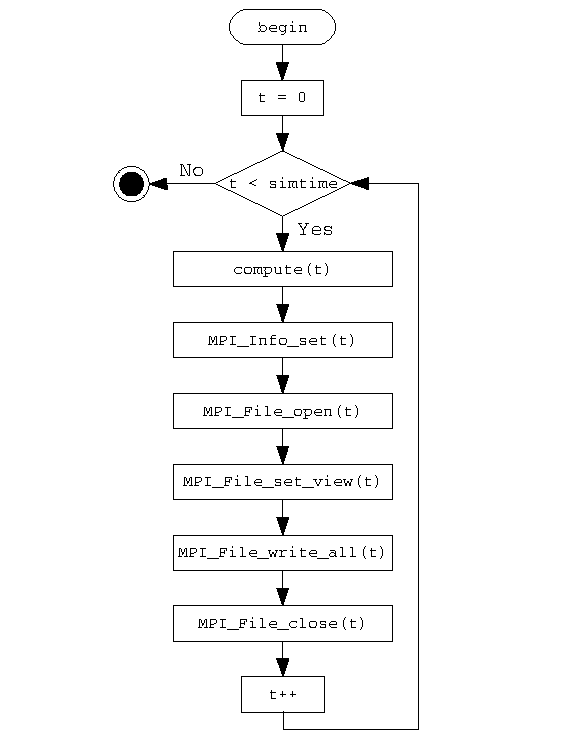
\includegraphics[width=0.5\columnwidth]{figures/workflow1}
%  \caption{}
%  \label{figure: workflow1}
%\end{figure}
%All the collective I/O routines in MPI-IO are blocking, that is, the implementation will return control to the application only when I/O is complete. The MPI-IO specifications also define a set of split collective I/O routines in which non-blocking collective I/O can be started using a `begin' function and completed using an `end' function. Nevertheless, the actual implementation supporting such features is currently missing and the overall application runtime is still highly dependent on I/O.

To take advantage of the proposed MPI-IO hint extensions, the application's workflow has to be modified. Figure~\ref{figure: workflow3} shows the classical application's workflow (cache disabled) as well as the modified version using the new hints (cache enabled). The difference %between Figure~\ref{figure: workflow1} and Figure~\ref{figure: workflow2} 
is that, in order to take advantage of the proposed hints and hide the cache synchronisation to the computation phase, the \codeword{MPI\_File\_close} for the I/O phase `k' %in Figure~\ref{figure: workflow2}
has been moved at the beginning of the I/O phase `k+1', just before the new file is opened.
%\begin{figure*}[!htb]
%  \centering
%  \begin{subfigure}{0.8\columnwidth}
%    \centering
%    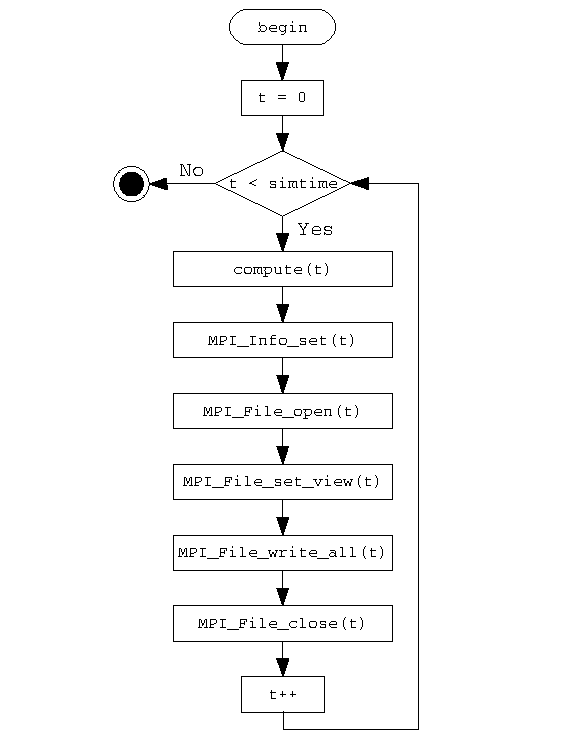
\includegraphics[width=\textwidth]{figures/workflow1}
%    \caption{\textit{}}
%    \label{figure: workflow1}
%  \end{subfigure}
%  \hspace*{0.25\columnwidth}%
%  \begin{subfigure}{0.8\columnwidth}
%    \centering
%    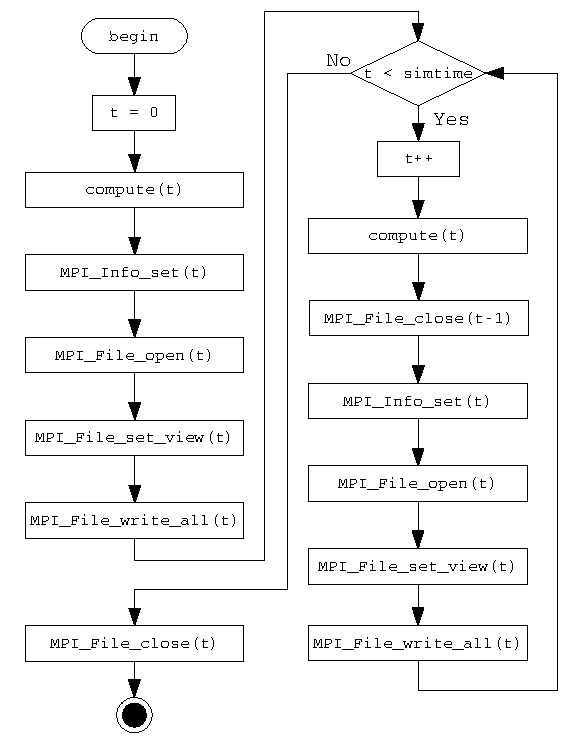
\includegraphics[width=\textwidth]{figures/workflow2}
%    \caption{\textit{}}
%    \label{figure: workflow2}
%  \end{subfigure}
%%  \hspace*{0.2\columnwidth}%
%  \caption{Classical application workflow (Figure~\ref{figure: workflow1}) and modified application workflow using the new MPI-IO hints (Figure~\ref{figure: workflow2}).}
%  \label{figure: workflow}
%\end{figure*}
\begin{figure}[!htb]
  \centering
  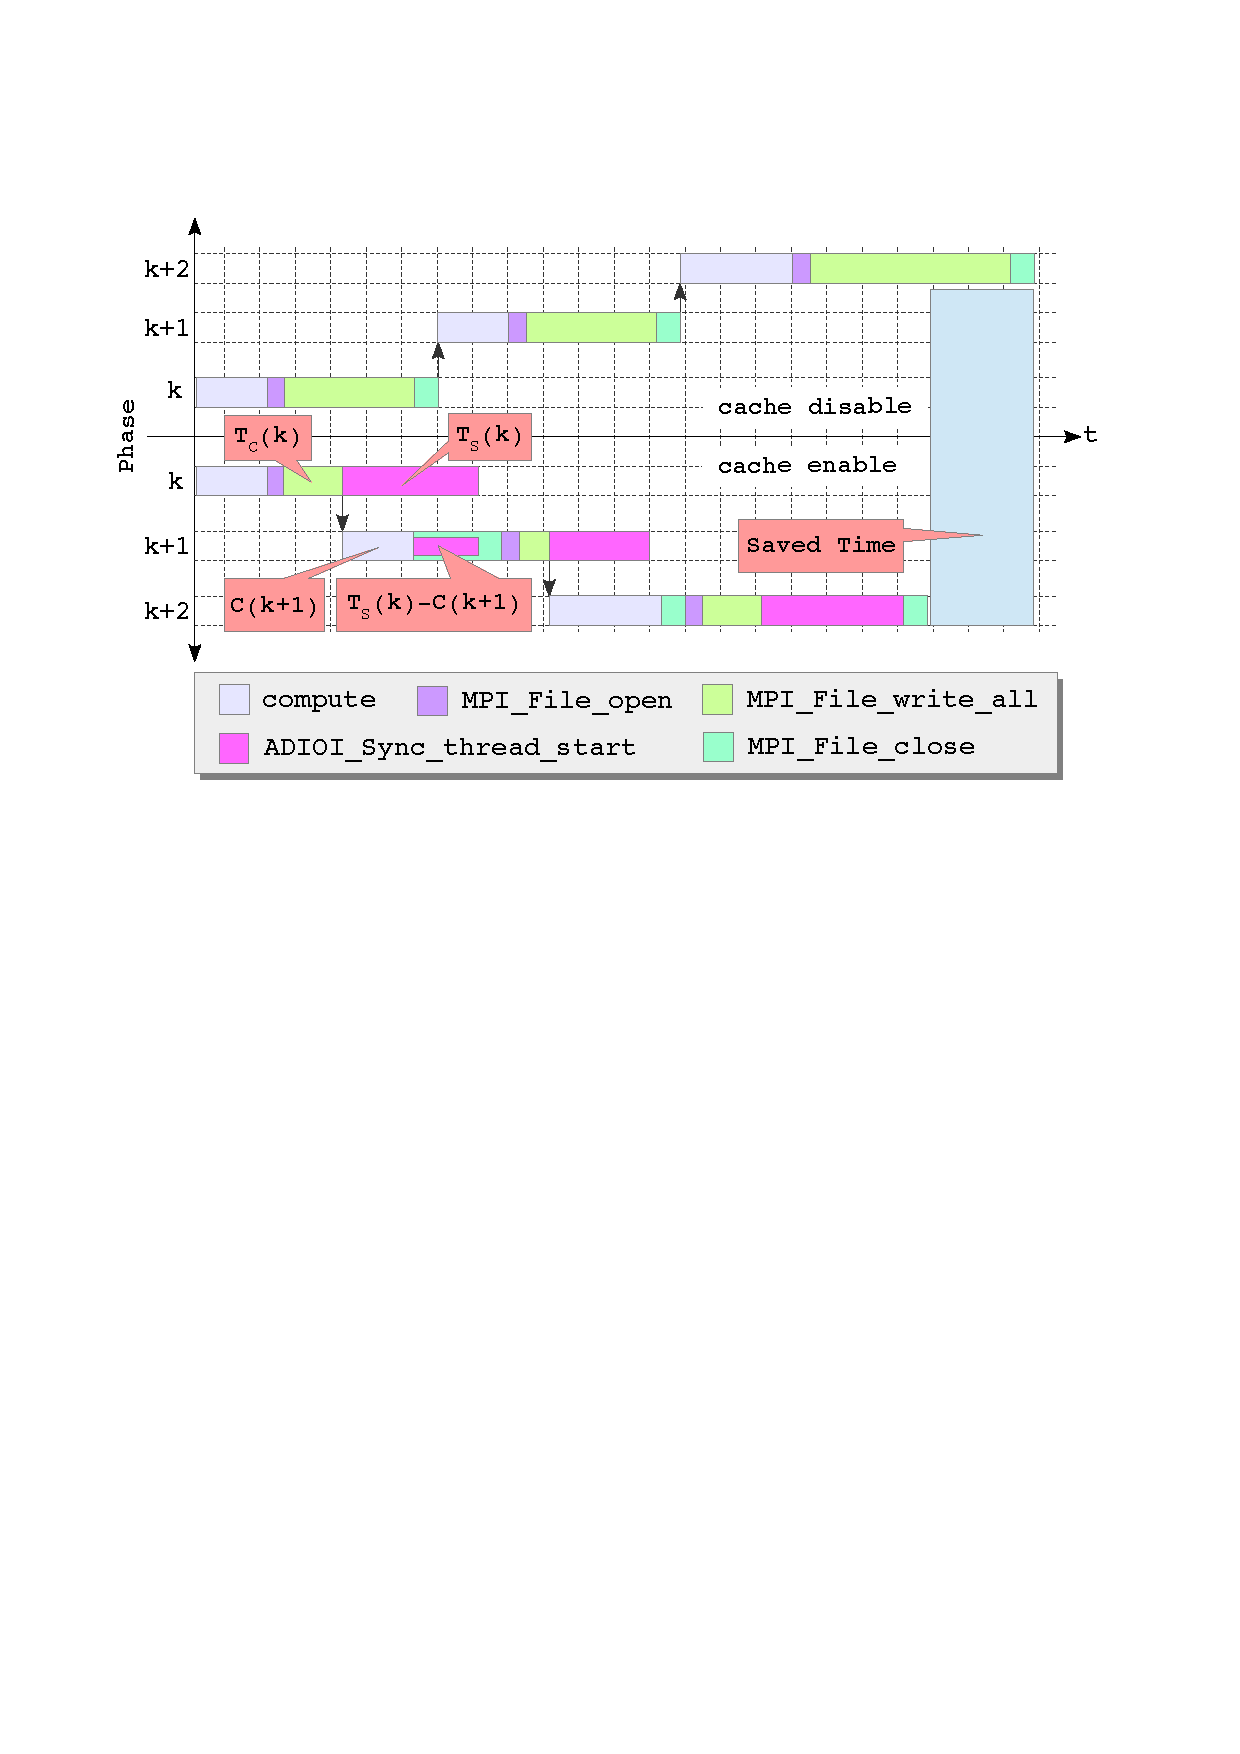
\includegraphics[width=0.96\columnwidth]{figures/workflow3}
  \caption{Standard and modified workflows. When cache is disabled, the next compute phase can start only after the previous file has been closed. When the cache is enabled the next compute phase can start immediately after data has been written to the cache. At the same time, background synchronisation of the cache file starts. When the new compute phase has completed, the file from the previous I/O phase is closed, forcing the implementation to wait for remaining data to be moved from the cache to the global file system.}
  \label{figure: workflow3}
\end{figure}

Since the workflow modification just presented might not be feasible for legacy applications, we developed a wrapper library that can reproduce this change behind the scenes. The wrapper library can be linked to the application or preloaded with \codeword{LD\_PRELOAD} and has been used for all the experiments contained in this paper. MPI-IO hints are defined in a configuration %file very much similar to an IOR hints file
and passed by the wrapper to \codeword{MPI\_File\_open}. %Unlike the IOR hints file mechanism,
We can define multiple hints targeting different files or groups of files. The library overloads \codeword{MPI\_\{Init,Finalize\}} and \codeword{MPI\_File\_\{open,close\}} using the PMPI profiling interface. The workflow modification can be triggered for a specific set of files (identified by the same base name) in the configuration file. Whenever one of such files is closed, our \codeword{MPI\_File\_close} implementation will return success. Nevertheless, the file will not be really closed. Instead, its handle will be kept internally for future references. When the next shared file with the same base name is opened, our \codeword{MPI\_File\_open} implementation will search for outstanding opened file handles and will invoke \codeword{PMPI\_File\_close} on them, this will trigger a cache synchronisation completion check for the file.
%Figure~\ref{figure: ext2ph-e10} shows how \codeword{ADIO\_WriteContigLocal} and \codeword{ADIO\_IfileSync} are integrated in the collective I/O implementation diagram previously introduced.
%\begin{figure}[!htb]
%  \centering
%  \includegraphics[width=\columnwidth]{figures/ext2ph-e10}
%  \caption{Integration of local write and synchronisation function in the collective I/O implementation.}
%  \label{figure: ext2ph-e10}
%\end{figure}

\subsection{I/O Bandwidth}
\label{subsec: bw-impr}
According to the new I/O workflow described in this section we have that, being $S(k)$ the amount of data to be written during the collective I/O operation of the phase `k', $T_c(k)$ the time needed to write $S(k)$ collectively to the cache using \codeword{MPI\_File\_write\_all}, $T_s(k)$ the time needed to synchronise (independently) the cached data in every aggregator to the global file system, using \codeword{ADIOI\_GEN\_IfileSync}, and $C(k+1)$ the computation time for the phase `k+1', the resulting I/O bandwidth for `k' is expressed by Equation~\ref{formula: bw}:

\begin{equation}\label{formula: bw}
        bw(k) = \frac{S(k)}{T_c(k) + max(0,\ T_s(k) - C(k+1))} \\
\end{equation}
Therefore, the total average bandwidth perceived by the application is:
\begin{equation}\label{formula: abw}
        BW = \frac{1}{N}\sum_{k=0}^{N-1}bw(k)
\end{equation}

From Equation~\ref{formula: bw} (in which we have considered the open time neglectable) it is clear that the maximum performance can be obtained when $C(k+1) \geq T_s(k)$, that is, when we can completely hide cache synchronisation by the computation phase. On the other hand when $C(k+1) < T_s(k)$ we might have a minima in the bandwidth since \codeword{MPI\_File\_close} needs to wait for cache synchronisation completion (Figure~\ref{figure: workflow3}). 
%Finally, being $T_g$ the standard collective write time to the global file system, we assume that $T_g >> T_c$. This assumption is legitimated by the fact that in very large scale systems the number of compute nodes (and thus the number of NVM devices) is orders of magnitude bigger than the available storage targets.
